%\part{The main loop}
%\frame{\partpage}

\begin{frame}{Basic game architecture}
    \begin{itemize}
        \item CPUs execute \textbf{sequences of instructions} \pause
            \begin{itemize}
                \item At the CPU level, there is no such thing as ``when $X$ happens, do $Y$'' \pause
                \item Instead: ``keep checking whether $X$ has happened; if so, do $Y$'' \pause
            \end{itemize}
        \item Thus games need to have a \textbf{main loop} \pause
        \item The main loop is usually part of the game's \textbf{engine} \pause
            \begin{itemize}
                \item Engines and high level frameworks (e.g.\ Kivy, Unity, Unreal)
                    usually implement the main loop for you \pause
                \item Low level frameworks (e.g.\ SDL, OpenGL, DirectX)
                    usually require you to implement your own main loop
            \end{itemize}
    \end{itemize}
\end{frame}

\begin{frame}{The basic main loop}
    The most basic main game loop does \textbf{three} things: \pause
    \begin{enumerate}
        \item Handle \textbf{input} \pause
            \begin{itemize}
                \item Mouse, keyboard, joypad etc. \pause
                \item Operating system events (minimise, close, alt+tab etc.) \pause
            \end{itemize}
        \item \textbf{Update} the state of the game \pause
            \begin{itemize}
                \item Physics, collision detection, AI etc. \pause
            \end{itemize}
        \item \textbf{Render} the game to the screen \pause
    \end{enumerate}
    It does these \textbf{once per frame} (typically 30 or 60 times per second) \pause
\end{frame}

\begin{frame}[fragile]{The basic main loop}
    \begin{lstlisting}
bool running = true;

while (running)
{
    handleInput();
    update();
    render();
}
    \end{lstlisting}
\end{frame}

\begin{frame}{Handling input}
    There are two ways of handling input in a game: \pause
    \begin{itemize}
        \item By responding to \textbf{events} \pause
            \begin{itemize}
                \item \lstinline{SDL_PollEvent} \pause
                \item See \url{https://wiki.libsdl.org/SDL_EventType} for a list of event types \pause
            \end{itemize}
        \item By querying \textbf{state} \pause
            \begin{itemize}
                \item \lstinline{SDL_GetKeyboardState}, \lstinline{SDL_GetMouseState},
                    \lstinline{SDL_GameControllerGetAxis}, etc. \pause
            \end{itemize}
    \end{itemize}
    What's the difference? \pause
    \begin{itemize}
        \item \textbf{Event}: ``The space bar was [pressed / released]'' \pause
        \item \textbf{State}: ``The space bar is [down / up] right now''
    \end{itemize}
\end{frame}

\begin{frame}{Updating the game state}
    \begin{itemize}
        \item Generally this is where your \textbf{game logic} is implemented \pause
        \item I.e.\ anything not directly related to input or graphics \pause
        \item What goes in here depends on the game...
    \end{itemize}
\end{frame}

\begin{frame}{Rendering}
    \begin{itemize}
        \item This is where you draw the \textbf{current state of the game} to the screen \pause
        \item Also draw any \textbf{heads-up display (HUD)} elements,
            e.g.\ score, lives, mini-map, etc. \pause
        \item Graphical effects (animations, particles) may be handled \textbf{either} in the render step
            \textbf{or} in the update step (but be consistent) \pause
        \item In frameworks like SDL, you generally \textbf{redraw everything} on every frame \pause
        \item Rendering in SDL is \textbf{double buffered} \pause
            \begin{itemize}
                \item \lstinline{SDL_Render}... functions actually draw to an
                    \textbf{off-screen buffer} \pause
                \item \lstinline{SDL_RenderPresent} displays the off-screen buffer on screen
            \end{itemize}
    \end{itemize}
\end{frame}

\begin{frame}{Screen refresh rate}
    \begin{itemize}
        \item Old CRT monitors worked by scanning an electron beam down the screen
            \begin{itemize}
                \item \url{https://www.youtube.com/watch?v=lRidfW_l4vs} \pause
            \end{itemize}
        \item Hence the term \textbf{(vertical) refresh rate} \pause
        \item Refresh rate is measured in \textbf{cycles per second} i.e.\ \textbf{Hz} \pause
        \item Other monitor technologies work differently, but still refresh the screen at regular intervals
    \end{itemize}
\end{frame}

\begin{frame}{Frame rate}
    \begin{itemize}
        \item We generally want to sync it up so that \newline
            \textbf{one display refresh = one main loop iteration} \pause
        \item If the main loop runs too slowly, we get ``lag'' \pause
        \item If the main loop runs too quickly, we waste resources on drawing things faster than the display can show them
    \end{itemize}
\end{frame}

\begin{frame}{Limiting the frame rate}
    \begin{itemize}
        \item If the renderer was created with the \lstinline{SDL_RENDERER_PRESENTVSYNC} flag,
            \lstinline{SDL_RenderPresent} waits for the next vertical blank \pause
        \item This limits the game's frame rate to the refresh rate of the device \pause
        \item However, refresh rates can vary \pause
            \begin{itemize}
                \item Older TVs: $\sim$ 30Hz
                \item HDTVs and standard monitors: 60Hz
                \item High-end ``gaming'' monitors: 120Hz or higher
            \end{itemize}
    \end{itemize}
\end{frame}

\begin{frame}{Limiting the update rate}
    \begin{itemize}
        \item Having the update frequency depend on the refresh rate would be bad! \pause
            \begin{itemize}
                \item The game could appear to run in slow or fast motion,
                    completely changing the gameplay \pause
            \end{itemize}
        \item This was the situation on older consoles:
            American/Japanese versions of games actually ran a little faster
            than European versions,
            due to the NTSC TV standard having a higher refresh rate than PAL!
    \end{itemize}
\end{frame}

\begin{frame}[fragile]{Variable time step}
    \begin{itemize}
        \item Have the update step depend on the \textbf{elapsed time since the last update} \pause
        \item Also known as the \textbf{delta time} \pause
        \item E.g.\ instead of this:
    \end{itemize}
    \begin{lstlisting}
player.positionX += player.velocityX;
    \end{lstlisting} \pause
    \begin{itemize}
        \item do this:
    \end{itemize}
    \begin{lstlisting}
player.positionX += player.velocityX * deltaTime;
    \end{lstlisting}
\end{frame}

\begin{frame}[fragile]{Measuring elapsed time}
    \begin{lstlisting}
bool running = true;
Uint32 lastFrameTime = SDL_GetTicks();

while (running)
{
    Uint32 currentTime = SDL_GetTicks();
    Uint32 deltaTime = currentTime - lastFrameTime;
    // deltaTime is the number of milliseconds since the last update
    
    handleInput();
    update(deltaTime);
    render();
    
    lastFrameTime = currentTime;
}
    \end{lstlisting}
\end{frame}

\begin{frame}{Variable time step}
    \begin{itemize}
        \item \textbf{Good:} the game will no longer run in slow or fast motion
            at different refresh rates \pause
        \item \textbf{Bad:} may increase the complexity of the \lstinline{update} function \pause
        \item \textbf{Bad:} some systems (e.g.\ physics) may become prone to numerical errors \pause
    \end{itemize}
\end{frame}

\begin{frame}{Fixed time step}
    \begin{itemize}
        \item Perform the update at a \textbf{fixed rate}, e.g.\ 60 times per second \pause
        \item If refresh rate $<$ 60Hz, update several times per frame \pause
        \item If refresh rate $>$ 60Hz, update once every few frames
    \end{itemize}
\end{frame}

\begin{frame}[fragile]{Fixed time step}
    \begin{lstlisting}
bool running = true;
Uint32 lastUpdateTime = SDL_GetTicks();
const Uint32 timePerUpdate = 1000 / 60;

while (running)
{
    Uint32 currentTime = SDL_GetTicks();
    handleInput();
    
    while (currentTime - lastUpdateTime >= timePerUpdate)
    {
        update();
        lastUpdateTime += timePerUpdate;
    }
    
    render();
}
    \end{lstlisting}
\end{frame}

\begin{frame}{Stalling}
    \begin{itemize}
        \item What if \lstinline{update} takes longer than \lstinline{timePerUpdate} to execute? \pause
        \item The \lstinline{while} loop will perform more and more iterations in an effort
            to catch up, eventually grinding the game to a halt \pause
        \item \textbf{Solution:} \lstinline{break} out of the loop after a maximum number of iterations
            (e.g.\ 10)
    \end{itemize}
\end{frame}

\begin{frame}{Interpolation}
    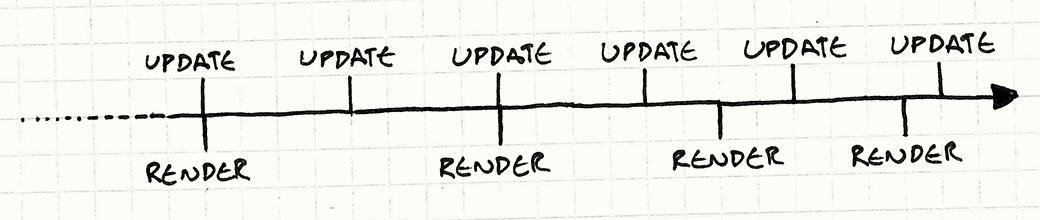
\includegraphics[width=\textwidth]{game-loop-timeline} \pause
    \begin{itemize}
        \item Rendering at ``irregular'' intervals (with respect to update) can result in
            jerky movement \pause
        \item Solution: \textbf{interpolate} between the two previous updates \pause
            \begin{itemize}
                \item E.g.\ if the render falls exactly halfway between two updates,
                    render each object exactly halfway between its positions
                    \textbf{before} and \textbf{after} the most recent update
            \end{itemize}
    \end{itemize}
\end{frame}

\begin{frame}{Further information on fixed time steps}
    \begin{itemize}
        \item \url{http://gafferongames.com/game-physics/fix-your-timestep/}
        \item \url{http://gameprogrammingpatterns.com/game-loop.html}
    \end{itemize}
\end{frame}

\begin{frame}{The ``main loop'' in Unity}
    \begin{center}
        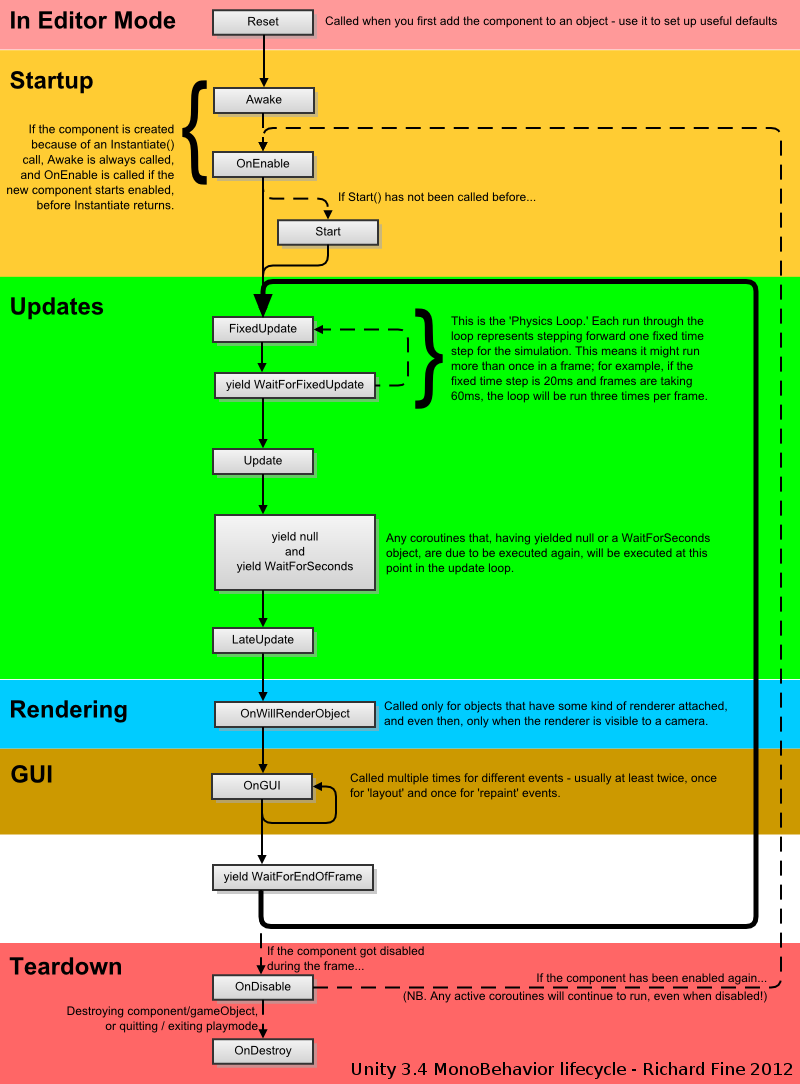
\includegraphics[height=0.8\textheight]{unity-lifetime}
    \end{center}
\end{frame}

\begin{frame}{Summary}
    \begin{itemize}
        \item The \textbf{main loop} of a game runs once per frame,
            and handles \textbf{input}, \textbf{updating} and \textbf{rendering}
        \item Using a \textbf{fixed time step} is a good idea, but be careful of \textbf{stalling}
    \end{itemize}
\end{frame}

